%! TEX root = ../main.tex
% ==============================================================
% IMMUTABLE — generated automatically, do not edit this block
%
% — Provenance ───────────────────────────────────────────────────
%   script            : analysis_scratch/wind_2s_vs_360s.py
%   computed_in       : analysis_scratch/wind_2s_vs_360s.py
%   plot_type         : wind_pre_paddle_psd
%   data_class        : DELEG
%   generated_at      : 2026-05-01T13:54:59
%   findings_doc      : (none)
%
% — Thesis context ──────────────────────────────────────────────
%   chapter           : 04
%   caption_label     : fig:ch04_wind_pre_paddle_psd
%   caption_short     : 
%
% — Filters ────────────────────────────────────────────────────
%   panel             : 
%   wind              : full
%   amplitude [V]     : 
%   frequency [Hz]    : 
%   probes            : 
%   run_category      : 
%   quality_flag      : 
%   mooring           : 
%
% — Data provenance ────────────────────────────────────────────
%   n_runs            : 
%   in_probes_used    : 
%   out_probes_used   : 
%   probe_configs     : 
%   non_final_config_n: 
%   datasets        :
%     PROCESSED-20251005-sixttry6roof-highMooring
%     PROCESSED-20251110-tett6roof-lowM-ekte580
%     PROCESSED-20251110-tett6roof-lowMooring
%     PROCESSED-20251110-tett6roof-lowMooring-2
%     PROCESSED-20251112-tett6roof
%     PROCESSED-20251113-tett6roof
%     PROCESSED-20251113-tett6roof-loosepaneltaped
%     PROCESSED-20251113-tett6roof-probeadjusted
%     PROCESSED-20260305-newProbePos-tett6roof
%     PROCESSED-20260306-newProbePos-tett6roof
%     PROCESSED-20260307-ProbPos4_31_FPV_2-tett6roof
%     PROCESSED-20260312-ProbPos4_31_FPV_2-tett6roof
%     PROCESSED-20260313-ProbePos4_31_FPV_2-tett6roof
%     PROCESSED-20260314-ProbePos4_31_FPV_2-tett6roof
%     PROCESSED-20260316-ProbePos4_31_FPV_2-tett6roof
%     PROCESSED-20260316-ProbePos4_31_FPV_2-tett6roof-under9Mooring
%     PROCESSED-20260319-ProbePos4_31_FPV_2-tett6roof-under9Mooring
%     PROCESSED-20260321-ProbePos4_31_FPV_2-tett6roof-under9Mooring-height100-RENAMED
%     PROCESSED-20260323-ProbePos4_31_FPV_2-tett6roof-under9Mooring-height100
%     PROCESSED-20260323-ProbePos4_31_FPV_2-tett6roof-under9Mooring-height136
%     PROCESSED-20260324-ProbePos4_31_FPV_2-tett6roof-under9Mooring-height100
%     PROCESSED-20260325-ProbePos4_31_FPV_2-tett6roof-under9Mooring-height100
%     PROCESSED-20260326-ProbePos4_31_FPV_2-tett6roof-under9Mooring-height100
%     PROCESSED-20260326-ProbePos4_31_FPV_2-tett6roof-under9Mooring-height100-lowrange
%     PROCESSED-20260327-ProbePos4_31_FPV_2-tett6roof-under9Mooring30-height100-lowrange
%   run_paths       :
%     (omitted — aggregate over > threshold runs, see datasets)
%
% — Method / numerical parameters ─────────────────────────────
%   grouper           : 
%   collapse_panels   : 
%   fft_window_hz     : 
%   extra_params      : Wind characterisation validation: does the 3 s pre-paddle window of a wave run reproduce the wind PSD measured on long (~31–381 s) nowave+fullwind runs? Canon datasets only (PROCESSED-20260326-*-lowrange + PROCESSED-20260327-*-lowrange — final probe config march2026_better_rearranging). Long-run set: 5 runs, durations 31, 33, 63, 360, 381 s. Per-long-run Welch PSD (Hann, nperseg = 8 s, linear detrend, Δf = 0.125 Hz) → 16–84 percentile envelope + median (green). Pre-paddle ensemble: first 3 s of all 70 fullwind+wave runs in the same datasets — safe because √(gh) = 2.39 m/s and the closest probe (8804 mm) sees no paddle motion before 3.68 s. Per-snippet single periodogram (Hann, linear detrend, Δf = 0.333 Hz) → 16–84 envelope + median (orange dashed). Probe shown: 9373/170 (IN, wall). Colour convention is local (green = long-run, orange = pre-paddle); does NOT use the thesis-wide WIND_COLOR_MAP because both curves represent the same wind condition (fullwind).
%
% — Summary stats cited in caption ────────────────────────────
%   stat:snippet_seconds : 3
%   stat:sigma_upstream_long_mm : 3.617
%   stat:sigma_upstream_snip_mm : 3.760
%   stat:sigma_upstream_delta_pct : +3.95
%   stat:Hs_upstream_long_mm : 14.467
%   stat:Hs_upstream_snip_mm : 15.039
%   stat:sigma_inWall_long_mm : 4.281
%   stat:sigma_inWall_snip_mm : 4.042
%   stat:sigma_inWall_delta_pct : -5.58
%   stat:Hs_inWall_long_mm : 17.122
%   stat:Hs_inWall_snip_mm : 16.167
%   stat:sigma_inFar_long_mm : 4.078
%   stat:sigma_inFar_snip_mm : 4.123
%   stat:sigma_inFar_delta_pct : +1.10
%   stat:Hs_inFar_long_mm : 16.314
%   stat:Hs_inFar_snip_mm : 16.492
%   stat:sigma_Out_long_mm : 0.360
%   stat:sigma_Out_snip_mm : 0.329
%   stat:sigma_Out_delta_pct : -8.61
%   stat:Hs_Out_long_mm : 1.439
%   stat:Hs_Out_snip_mm : 1.317
%
% — Subfigures available ───────────────────────────────────────
%     FIGURES/ch04_wind_pre_paddle_psd.pdf
% ── end immutable block ─────────────────────────────────────────
\begin{figure}[htbp]
  \centering
  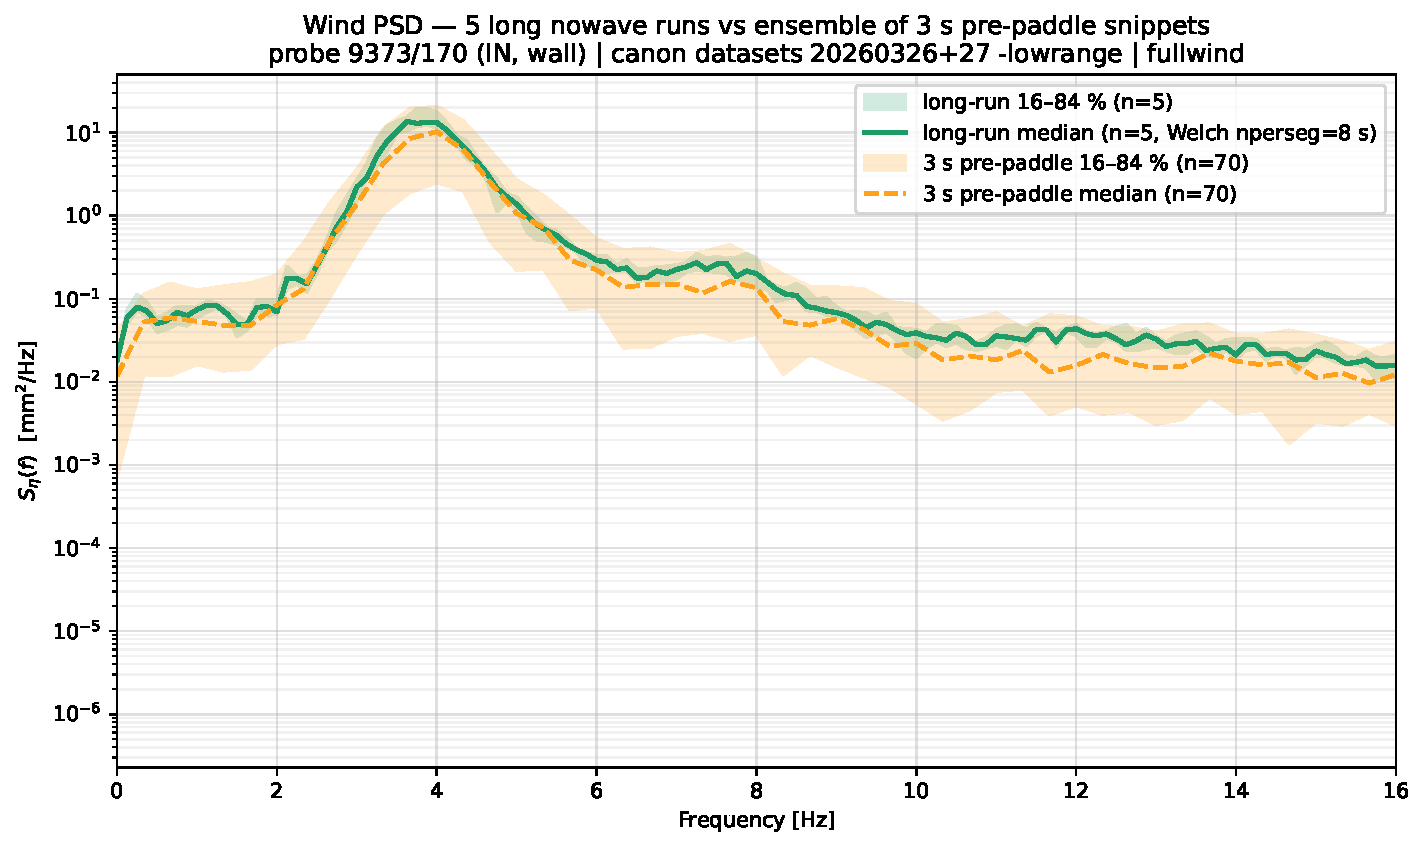
\includegraphics[width=\linewidth]{FIGURES/ch04_wind_pre_paddle_psd.pdf}
  \caption{
    % TODO: write caption
  }
  \label{fig:ch04_wind_pre_paddle_psd}
\end{figure}
